\documentclass{standalone}

\usepackage{tikz}

\begin{document}
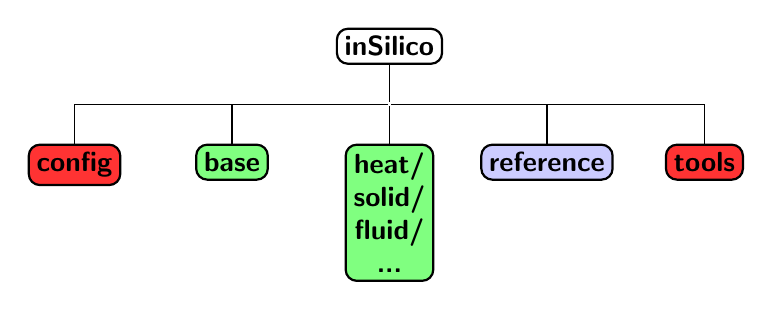
\begin{tikzpicture}
  
  \node[anchor=center,inner sep=-1mm] (X) at (0,0) {};

  % node styles
  \tikzstyle{Box}=[
  anchor=north,
  thick,
  font=\sffamily\bfseries,
  align=center,
  inner sep=1mm,
  shape=rectangle,rounded corners,draw]

  \tikzstyle{Label}=[font=\sffamily\bfseries\tiny]

  \draw (X) node[Box,anchor=south] (I)  at +( 0.0,  0.5) {inSilico};

  \draw (X) node[Box,fill=  red!80] (C)  at +(-4.0, -0.5) {config};
  \draw (X) node[Box,fill=green!50] (B)  at +(-2.0, -0.5) {base};
  \draw (X) node[Box,fill=green!50] (M)  at +( 0.0, -0.5) {heat/\\solid/\\fluid/\\...};
  \draw (X) node[Box,fill= blue!20] (R)  at +( 2.0, -0.5) {reference};
  \draw (X) node[Box,fill=  red!80] (T)  at +( 4.0, -0.5) {tools};

  \draw (I.south) -- (X) -- +(-2,0) -- (B.north);
  \draw (X) ++(-2,0) -- +(-2,0) -- (C.north);
  \draw (X) -- (M.north);
  \draw (X) -- +(2,0) -- (R.north);
  \draw (X) ++(2,0) -- +(2,0) -- (T.north);

\end{tikzpicture}
\end{document}


%%% Local Variables: 
%%% mode: latex
%%% TeX-master: t
%%% End: 
